\chapter{DESC: A Distributed Event Stream Composition system}
\label{ch4}
\textit{This chapter presents DESC, a distributed event streams composition system that deals with QoS. It presents the general architecture of the system, and defines its main components.}
\vspace{5cm}
\vspace{2ex}\vfill
\minitoc

%\section{Introduction}
%In Chapter \ref{ch3}, we presented a model for event streams composition with quality of service. This chapter presents a distributed event composition system (DESC) that implements the proposed model as a network of operators executed by distributed event processing units.
%The 

\section{General architecture / Event processing network}
The general vision of our QoS based complex event processing system can be briefly described as follows: applications subscribe to composite events by issuing complex event patterns to the system, with associated QoS requirements. The system then deploys a set of distributed event processing units, which apply different strategies to meet QoS requirements during event processing. The complex events generated by the event processing units are notified to consumers. In a smart grid, such an infrastructure can act as a middleware on which utility applications can rely for detecting interesting or critical situations (sensors errors, alarms, etc.) over the electrical grid, with some QoS guarantees (e.g., priority, notification latency, etc.).
\begin{figure}[htbp]
  %\vspace{-0.2cm}
  \centering
   {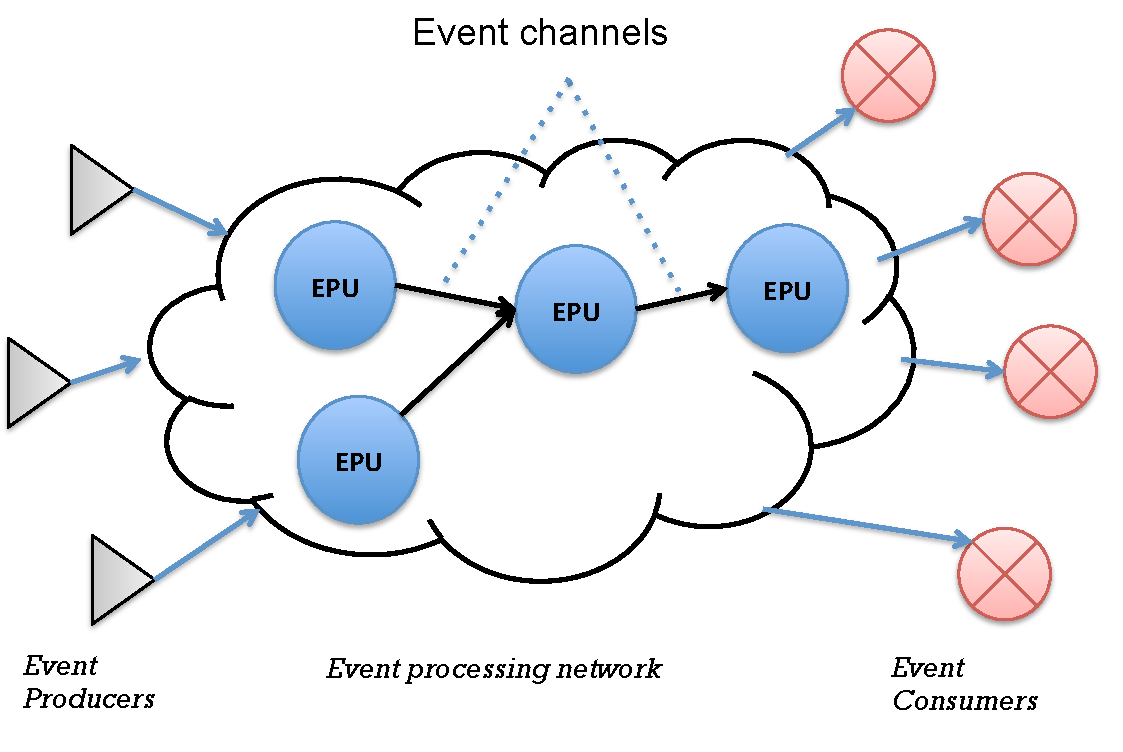
\epsfig{file = chap4/images/epn.pdf, width = 3in}}
  \caption{Event processing network}
  \label{fig:epn}
 \end{figure}

\section{Event producer}
An event producer is a component able to generate events. This can be a physical device such as a sensor, or a software component. The definition of an event producer includes its ID, a brief description, its location, and at the type of events it generates with their associate priority. A producer generates events with respect to a production rate. A production rate is defined by a probability distribution.

Producer P:= <ID, description, location, eventType, priority, productionRate> 

\section{Quality of service}
 \label{ch4:sec-three}
 Event streams composition in smart grids face many challenges that are due to QoS that have to be guaranteed. This section first discusses such QoS requirements and then, presents how they are modeled as QoS expressions.              
\subsection{QoS dimensions}
The quality of service dimensions that we identify as relevant for smart grids are:
\begin{itemize}
 \item \textit{Latency}. Once detected, events may have to be notified as fast as possible to consumers. Such a timing constraint is even critical in some applications. For example, in the common practice for power device protection, the circuit breaker must be opened immediately if the voltage or current on a power device exceeds the normal values. The notification latency of an event is the time elapsed between its production and its notification to interested consumers.
 \item \textit{Event priority}. Event priority defines a priority order between events. In some contexts, there may exist priorities between events that have to be captured by the event processing runtime. For example in a smart grid, alarm events are generally higher priority than events that report energy consumption. Events that have a higher priority have to be processed and notified earlier than less priority events.
 \item \textit{Memory occupation}. Different devices may have different available memory capacities. To adapt the event processing to the memory capacity of each device, it must be a way to specify the maximum memory occupation incurred by an event processing unit at the execution time. The memory occupation constraint gives an upperbound on the number of events that an event processing unit can maintain in its main memory at execution time.
\end{itemize}

\subsection{QoS expression}
Let's consider three domains $D_{latency}$, $D_{priority}$, $D_{memory}$, corresponding to the QoS dimensions latency, event prioity and memory occupation respectively.
Those domains are described below:
%The domains corresponding to the QoS criteria we considered are described below:
\begin{itemize}
 \item $D_{latency} \subseteq R+$, as the latency corresponds to a time delay (an expected value for measuring time belongs to the set of positive real numbers). The domain inherits the properties of R+ (e.g. the operators of comparison). Best is shortest for latencies, the latency is bounded with the comparison operator ``less than'' (<) and ``less or equal to'' ($\leq$). 
 \item $D_{priority} \subseteq N^*$. An event type is associated to a priority level. The lower is the priority level, the higher is the priority associated to the event. The priority level varies according to the event type. The domain inherits the properties of $N$ (e.g. the operators of comparison). 
 The priority is heavily restricted bounded, thus ``equal to'' (=) is the only accepted comparison operator.
 \item $D_{memory}  \subseteq N$, as the memory corresponds to a quantity. The domain inherits the properties of $N$. The memory occupation is associated to an upper-bound that indicates the maximum memory available on a processing device. This is denoted by the comparison operator ``less or equal to'' ($\leq$).  
\end{itemize}
Let us assume $D$ the set of the QoS domains that we considered, that is $D = D_{latency} \bigcup D_{priority}$ $ \bigcup D_{memory}$.
Given a domain $D_Q$, we assume a function \textit{name($D_Q$)} that returns its  name, a function \textit{operator($D_Q$)} that returns the set of related operators, and a function \textit{value($D_Q$)} that returns the set of included values.
For instance, let us consider the domain $D_{priority}$, thus: 
\begin{itemize}
 \item \textit{name($D_{piority}$)} = event priority,
 \item \textit{operator($D_{priority}$)} = { equal to (=) },
 \item \textit{value($D_{latency}$)} = $N^*$, this is the set of all positive integer numbers.
\end{itemize}
Let also consider that $\mathcal{L}$ is the set of available processing devices.
\subsubsection{Atomic QoS expression} 
An atomic QoS expression is of the form $(d, \theta, v)$ or , $(d, \theta, v, l)$ where 
\begin{itemize}
 \item d denotes a domain $D_Q , D_Q \in D$,
 \item $\theta \in$ \textit{operator($D_Q$)},
 \item $v \in$ \textit{value($D_Q$)},
 \item $l \in \mathcal{L}$ is a processing device.
\end{itemize}
For instance, the atomic QoS (latency, $\leq$, 2000) specifies that the latency for notifying an event must be less or equal to 2000 ms, assuming that the time unit is the millisecond. In the same way, the atomic QoS (memory, $\leq$, 1000, device1) specifies that the memory occupation on the device ``device1'' must be less or equal to 1000 Mo, assuming that the unit for the memory is the megabyte.  

\subsubsection{Complex QoS expression} 
A complex QoS expression specifies multiple QoS criteria. It is defined inductively as follows.
\begin{enumerate}
 \item An atomic QoS is a complex QoS expression.
 \item If $QC_1$ and $QC_2$ are complex QoS expressions then $QC_1 \wedge QC_2$ is a complex QoS expression.
\end{enumerate}
 The QoS expression (latency, $\leq$, 2000) $\wedge$ (event priority, =, 1) specifies that the latency must be less than or equal to 2000 ms, and in addition, the highest priority level (i.e. priority = 1) is required.
%Dmemocc domain represent the memory occupation criterion;  Dmemocc ⊆ N ≤ m. Where  m corresponds to the maximum memory capacity of the current device. The domain inherits the properties of N. The event processing memory occupation has an upper-bound of the the number of events that an event processing unit can maintain, it is denoted by the comparison operator ‘less than or equal to’ (≤).
